\documentclass[border=2pt]{standalone}
\usepackage{tikz}
\usepackage{amsmath}
\begin{document}
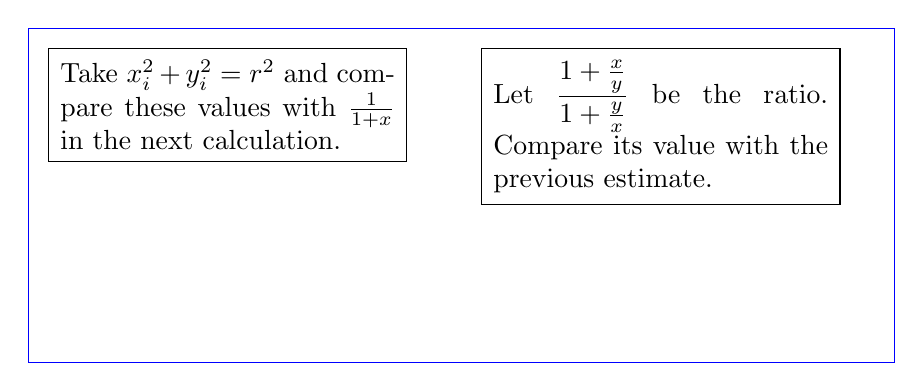
\begin{tikzpicture}
  \draw[blue] (-.25,-4) rectangle (10.75,.25);
  \node[draw,anchor=north west,inner sep=1ex] at (0,0) {
    \begin{minipage}{4.25cm}
      Take $x_i^2 + y_i^2 = r^2$ and compare these values with
      $\frac{1}{1+x}$ in the next calculation.
    \end{minipage}
  };
  \node[draw,anchor=north west,inner sep=1ex] at (5.5,0) {
    \begin{minipage}{4.25cm}
      Let $\displaystyle\frac{1+\frac{x}{y}}{1+\frac{y}{x}}$ be the ratio.
      Compare its value with the previous estimate.
    \end{minipage}
  };
\end{tikzpicture}
\end{document}
